\chapter{Implementierung \& Test}
\label{chap: Implementierung und Test}
In diesem Kapitel wird beschrieben wie das im Kapitel \ref{chap: Konzept} vorgestellte Konzept in der Bibliothek \textit{gedcom7.js} implementiert wird. 

%========================================================================================
% SECTION: GEDCOM GRAMMATIK
%========================================================================================
% Reihenfolge Grammatik & Grammatik Generator??
\section{Gedcom Grammatik}
\label{sec: Implementierung - Gedcom Grammatik}
% zeigen wie eine Grammatik aussieht
% Zeigen wie der Postprocessor funktioniert (auch Ausschnitt von Lexer möglich)
% Problem mit Ambigious Grammar -> erklären was das Problem ist und wie gelöst wurde
\subsection{Gedcom7 Syntax in Nearley}
\label{subsec: Implementierung - Gedcom Grammatik - Gedcom7 Syntax in Nearley}
Da die Gedcom7- sowie die Nearley Syntax beide auf EBNF-Sprachkonzepten basieren, lässt sich die Gedcom7 Spezifikation ohne weiteres in eine Nearley Grammatik übersetzten. Um Nearley Regeln für eine \textit{Gedcom Line}\footnote{siehe \hyperref[sec: GEDCOM Version 7]{Kapitel GEDCOM Version 7}} zu definieren, können die folgenden Tokens für das Leerzeichen, den \textit{Cross-Reference Identifier} und die End-Of-Line Zeichenfolge in Form von regulären Ausdrücken definiert werden:
\\ \\
\begin{minipage}{1.0\textwidth} \small
	\begin{lstlisting}
		D    : /[ ]/
		Xref : /\@[A-Z0-9\_]+\@/	
		EOL  : /(?:\r\n?|\n)/
	\end{lstlisting}
	\captionof{lstlisting}{Tokens für eine Gedcom Line, definiert als regulärer Ausdruck }
	\label{lst: tokens gedcom line}
\end{minipage}
\\ \\
Diese regulären Ausdrücke werden in der Vorverarbeitungsphase vom Moo-Lexer verwendet, um zusammenhängende Zeichen zu Tokens zu gruppieren, die dann in der Nearley Grammatik über den Tokennamen mit einem vorangestellten \%-Zeichen angesprochen werden können. Soll nun die erste Line eines Family-Records geparsed werden, könnte dies mit der folgenden Nearley-Regel umgesetzt werden:
\\ \\
\begin{minipage}{1.0\textwidth} \small
	\begin{lstlisting}
		record_FAM -> "0"  %D  %Xref  %D  "FAM"  %EOL 
	\end{lstlisting}
	\captionof{lstlisting}{Nearley Regel zum parsen eines Family Records}
	\label{lst: nearley regel family record first line}
\end{minipage}
\\ \\
Diese Regel akzeptiert eine Line mit dem Level 0, einem syntaktisch korrekten Cross-Reference-Identifier, dem Tag \textit{FAM} gefolgt von einem EOL-Token. Getrennt werden die Bestandteile durch ein Leerzeichen. 


Sollen nun ebenfalls HUSB- und WIFE Structures als Substructures des Family Records akzeptiert werden, könnte die Nearley Grammatik wie folgt erweitert werden:
\\ \\
\begin{minipage}{1.0\textwidth} \small
	\begin{lstlisting}
		record_FAM
			-> "0"  %D  %Xref  %D  "FAM"  %EOL 
			|  record_FAM  record_FAM_Substructs:+
		
		record_FAM_Substructs 
			-> "1"  %D  "HUSB"  %D  %Xref  %EOL
			|  "1"  %D  "WIFE"  %D  %Xref  %EOL 
	\end{lstlisting}
	\captionof{lstlisting}{Nearley Regel zum parsen eines Family Records mit HUSB- und WIFE Substructures}
	\label{lst: nearley regel family record with husb and wife}
\end{minipage}
\\ \\
Auf diese Weise nimmt würde der Nearley Parser einen Family Record ohne Substructures und einen Family Record mit beliebig vielen Substructures (in diesem Fall HUSB- und WIFE Structures) als Eingabe akzeptieren. Sollen nun die weiteren Lines aus Listing \ref{lst: family record example} ebenfalls in die Grammatik aufgenommen werden, müssen Regeln für die Datentypen der Payloads des MARR-Events und der NCHI-Structure definiert werden. Die Anzahl der Kinder wird als  \textit{Integer} Datentyp kodiert, also ein Folge von Dezimalziffern. Nach der Gedcom7 Spezifikation dürfen \textit{Integer} Werte nicht leer sein und führende Nullen sind erlaubt, sollten aber vermieden werden. Eine Regel für den Datentyp \textit{Integer} kann also dargestellt werden als
\\ \\
\begin{minipage}{1.0\textwidth} \small
	\begin{lstlisting}
		digit    ->  [0-9]
		Integer  ->  digit:+
	\end{lstlisting}
	\captionof{lstlisting}{Nearley Regel für den Datentyp \textit{Integer}}
	\label{lst: nearley regel integer}
\end{minipage}
\\ \\ 
Für das MARR-Event, also die Hochzeit der Ehepartner der Familie, ist eine \textit{DATE Structure} zum Festhalten des Datums der Hochzeit hinterlegt. Dieses Datum wird mit dem Datentyp \textit{DateValue} kodiert, der im Gegensatz zum \textit{Integer} wesentlich mehr Regeln umfasst. Ein \textit{DateValue} kann auf vier verschiedene Weisen dargestellt sein:
\begin{enumerate}
	\item \textit{date}: Ein mehr oder weniger genau spezifiziertes Datum, z.B. ``JULIAN 13 MAR 1998 BCE''
	\item \textit{datePeriod}: Ein Zeitintervall, dass von einem Startdatum bis zu einem Enddatum angegeben wird, z.B. ``FROM 15 FEB 2001 TO 23 MAR 2001''
	\item \textit{dateRange}: Ein ungenaueres Zeitintervall, bei dem nur Grenzen angegeben werden, z.B. ``BET 15 FEB 2001 AND 23 MAR 2001''
	\item \textit{dateApprox}: Eine Schätzung des Datums (ABT x: genaues Datum unbekannt, aber nahe x), z.B. ``ABT 15 FEB 2001''
\end{enumerate}
Diese Zusammenhänge ergeben die folgenden Nearley Regeln für die Definition des Datentyps \textit{DateValue}:
\\ \\
\begin{minipage}{1.0\textwidth} \small
	\begin{lstlisting}
		DateValue   ->  (date | DatePeriod | dateRange | dateApprox):?
		
		date        ->  (calendar  D):?  
						((day  D):?  month  D):?  
						year  
						(D  epoch):?
		datePeriod  ->  ("FROM"  D  date  D):?  "TO"  D  date
		dateApprox  ->  ("ABT" | "CAL" | "EST")  D  date 
		dateRange   ->  "BET"  D  date  D  "AND"  D  date  
					|   "AFT"  D  date  
					|   "BEF"  D  date 
		
		calendar ->  "GREGORIAN" | "JULIAN" | "FRENCH_R" | "HEBREW"
		day      ->  Integer  
		year 	 ->  Integer
		month    ->  Tag
		epoch    ->  "BCE" | Tag
		
		Tag 	 ->  upperCaseLetter  |  digit  |  underscore 
	\end{lstlisting}
	\captionof{lstlisting}{Nearley Regel für den Datentyp \textit{DateValue}}
	\label{lst: nearley regel date}
\end{minipage}
\\ \\ 
Werden all diese Regeln zusammengefasst lässt sich die folgende Grammatik definieren, die den Family Record aus Listing \ref{lst: family record example} als Eingabe akzeptiert:
\\ \\
\begin{minipage}{1.0\textwidth} \small
	\begin{lstlisting}
		record_FAM_Substructs
			-> "0"  %D  %Xref  %D  "FAM"  %EOL 
			|  record_FAM  record_FAM_Substructs:+
		
		record_FAM_Substructs 
			-> "1"  %D  "HUSB"  %D  %Xref  %EOL
			|  "1"  %D  "WIFE"  %D  %Xref  %EOL 
			|  "1"  %D  "NCHI"  %D  Integer  %EOL 
			|  structure_MARR 
		
		structure_MARR
			-> "1"  %D  "MARR" %EOL
			|  structure_MARR  
		
		structure_DATE
			-> "2" %D  "DATE"  %D  DateValue  %EOL
	\end{lstlisting}
	\captionof{lstlisting}{Nearley Grammatik für den Family Record aus Listing \ref{lst: family record example}}
	\label{lst: vollständige nearley grammatik family record}
\end{minipage}
\\ \\ 
Mit diesem Vorgehen können Nearley Regeln für alle Datentypen, Structures und Records definiert werden, die zu einer Grammatik für die Syntaxüberprüfung von Gedcom7 Dateinen zusammengesetzt werden können.


\subsection{Nearley Postprozessor}
\label{subsec: Implementierung - Gedcom Grammatik - Nearley Postprozessoren}
Der Nearley Postprozessor für die Bibliothek \textit{gedcom7.js} enthält 3 Funktionen: 

\vspace{1em}
\textsc{\textbf{joinAndUnpackAll()}:} \vspace{0.5em} \\
Wie in Abschnitt \ref{subsec: Konzept - Gedcom Grammatik - Pre- und Postprozessor} beschrieben, überführt ein \textit{Nearley-Parser} jedes Zeichen, das mit einer Regel übereinstimmt, in ein Array. Bei komplexeren Grammatiken wie der Gedcom7 Spezifikation führt dies dazu, dass sehr viele Arrays innereinander verschachtelt werden, sodass schnell hohe Verschatlungsgrade erreicht werden. Ein Beispiel hierfür wäre der in Abschnitt \ref{subsec: Implementierung - Gedcom Grammatik - Gedcom7 Syntax in Nearley} definierte Datentyp \textit{DateValue}. Hier würde jeder Bestandteil eines DateValues in ein eigenes Array verschachtelt werden. Wird beispielsweise das Datum 
\begin{center}
	13 MAR 1998 BCE
\end{center}
ohne Postprozessoren verarbeitet, wird das Array
\begin{center}
	[13, , [MAR, , [1998, , [BCE, , ]]]]
\end{center}
zurückgegeben, dass eine Weiterverarbeitung sehr umständlich macht. Daher wird der Postprozessor \textsc{joinAndUnpackAll()} implementiert, der über die JavaScript Funktion \textit{flat()} alle Elemente des Arrays rekursiv verkettet und anschließend über die Funktion \textit{join()} zu einer Zeichenkette zusammenfügt. Wird dieser Postprozessor einem Datentyp wie \textit{DateValue} zugewiesen, wird jedes syntaktisch korrekte Datum als Zeichenkette zurückgegeben und kann so direkt als LineValue für die weitere Verarbeitung verwendet werden. Die in Listing \ref{lst: nearley regel date} definierte Regel würde sich ergeben zu
\\ \\
\begin{minipage}{1.0\textwidth} \small
	\begin{lstlisting}
		DateValue   
			->  (date | DatePeriod | dateRange | dateApprox):?
				
	\end{lstlisting}
	\captionof{lstlisting}{Erweiterung der Nearley Regel für den Datentyp \textit{DateValue}}
	\label{lst: nearley regel date mit postprozessor}
\end{minipage}
\\ \\

\vspace{1em}
\textsc{\textbf{createStructure()}:} \vspace{0.5em} \\
Der Postprozessor \textsc{createStructure()} wird verwendet, um die gelesene Line mit Structure Informationen anzureichern. In der Nearley Regel wird die Line selbst, der Typ und die in der Gedcom7 Spezifikation definierte URI der Line und die Structures bei denen eine Kardinalitätsüberprüfung notwendig ist an den Postprozessor übergeben. Für den in Listing \ref{lst: vollständige nearley grammatik family record} Family Record ergibt sich der Postprozessoraufruf wie folgt:
\\ \\
\begin{minipage}{1.0\textwidth} \small
	\begin{lstlisting}
		record_FAM
			-> "0"  %D  %Xref  %D  "FAM"  %EOL
			
	\end{lstlisting}
	\captionof{lstlisting}{Nearley Regel zum parsen eines Family Records mit Postprozessor}
	\label{lst: nearley regel family record mit postprozessor}
\end{minipage}
\\ \\
Im Parameter \textit{checkCardinalityOf} werden die URIs alle Structures angegeben, bei denen eine Kardinalitätsüberprüfung notwendig ist und die in der Gedcom7 Spezifikation definierte Kardinalität als Wert zugewiesen. Kardinalitätsüberprüfungen sind bei allen Substructures erforderlich, die für die SUperstructure als notwendig definiert wurden (1:1 und 1:M) oder für die eine Maximale Anzahl festgelegt ist (also 0:1 und 1:1). In der Funktion \textsc{createStructure()} werden alle Informationen abhängig vom übergebenen Type zusammengefasst und als JavaScript Objekt an den Parser zurückgegeben. Für einen Family Record ergibt sich die Funktion zu:
\\ \\
\begin{minipage}{1.0\textwidth} \small
	\begin{lstlisting}
	createStructure: (params) => {
		// create line object depending on type of line
		let lineObject = {};
		lineObject = { 
			level: line[0], 
			xref: line[2], 
			tag: line[4], 
			lineVal: '', 
			EOL: line[5] 
		};
		
		// return data object with structure information
		return {
			uri: params.uri,
			line: lineObject,
			type: params.type,
			lineValType: params.lineValType || null,
			superstructFound: false,
			substructs: [],
			checkCardinalityOf: params.checkCardinalityOf
		};
	}
	\end{lstlisting}
	\captionof{lstlisting}{Funktion \textsc{createStructure()} für einen Family Record}
	\label{lst: createStructure für Family Record}
\end{minipage}
\\ \\

\vspace{1em}
\textsc{\textbf{addSubstructure()}:} \vspace{0.5em} \\
Die zusammengesetzte Regel ergibt sich zu 
\\ \\
\begin{minipage}{1.0\textwidth} \small
	\begin{lstlisting}
		record_FAM
			-> "0"  %D  %Xref  %D  "FAM"  %EOL
			
	\end{lstlisting}
	\captionof{lstlisting}{Vollständige Nearley Regel zum parsen eines Family Records mit Substructures}
	\label{lst: nearley regel family record mit postprozessor und substructs}
\end{minipage}
\\ \\

%========================================================================================
% SECTION: GRAMMATIK GENERATOR
%========================================================================================
\section{Grammatik Generator}
\label{sec: Implementierung - Grammatik Generator}
Der in Abschnitt \ref{sec: Konzept - Grammatik Generator} vorgestellte Grammatik Generator wird über die Klasse \textsc{GrammarGenerator}, wie in Abbildung \ref{fig: UML Klassendiagramm GrammarGenerator} dargestellt, implementiert. Über die Klassenmethode \textit{build(path)} kann eine Instanz von \textsc{GrammarGenerator} erstellt werden, der die Gedcom Grammatik an dem mit dem Parameter \textit{path} spezifizierten Pfad erzeugt. Bei der Instanzerzeugung wird im ersten Schritt der Nearley-Header, der in der Nearley Datei \textit{NearleyHeader.ne} spezifiziert ist, eingelesen und als Instanzvariable in Form einer Zeichenkette gespeichert. Dieser Nearley-Header stellt den obersten Eintrag jeder Nearley-Datei dar, die vom \textsc{GrammarGenerator} erzeugt wird und enthält die Include-Statements für Datentypen, Postprozessoren, etc. und den Aufruf des Moo-Lexers. Anschließend werden die Gedcom Grammatik Definition, die in Form von JavaScript Objekten gespeichert sind, gelesen und gespeichert. Anschließend kann diese Gedcom Grammatik Definition mit der Funktion \textit{generateGrammar()} in Nearley-Dateien überführt werden, die dann zu Nearley Parsern kompiliert werden können. In den folgenden Kapitel wird auf diese Schritte im Detail eingegangen.
\begin{figure}[h]
	\centering
	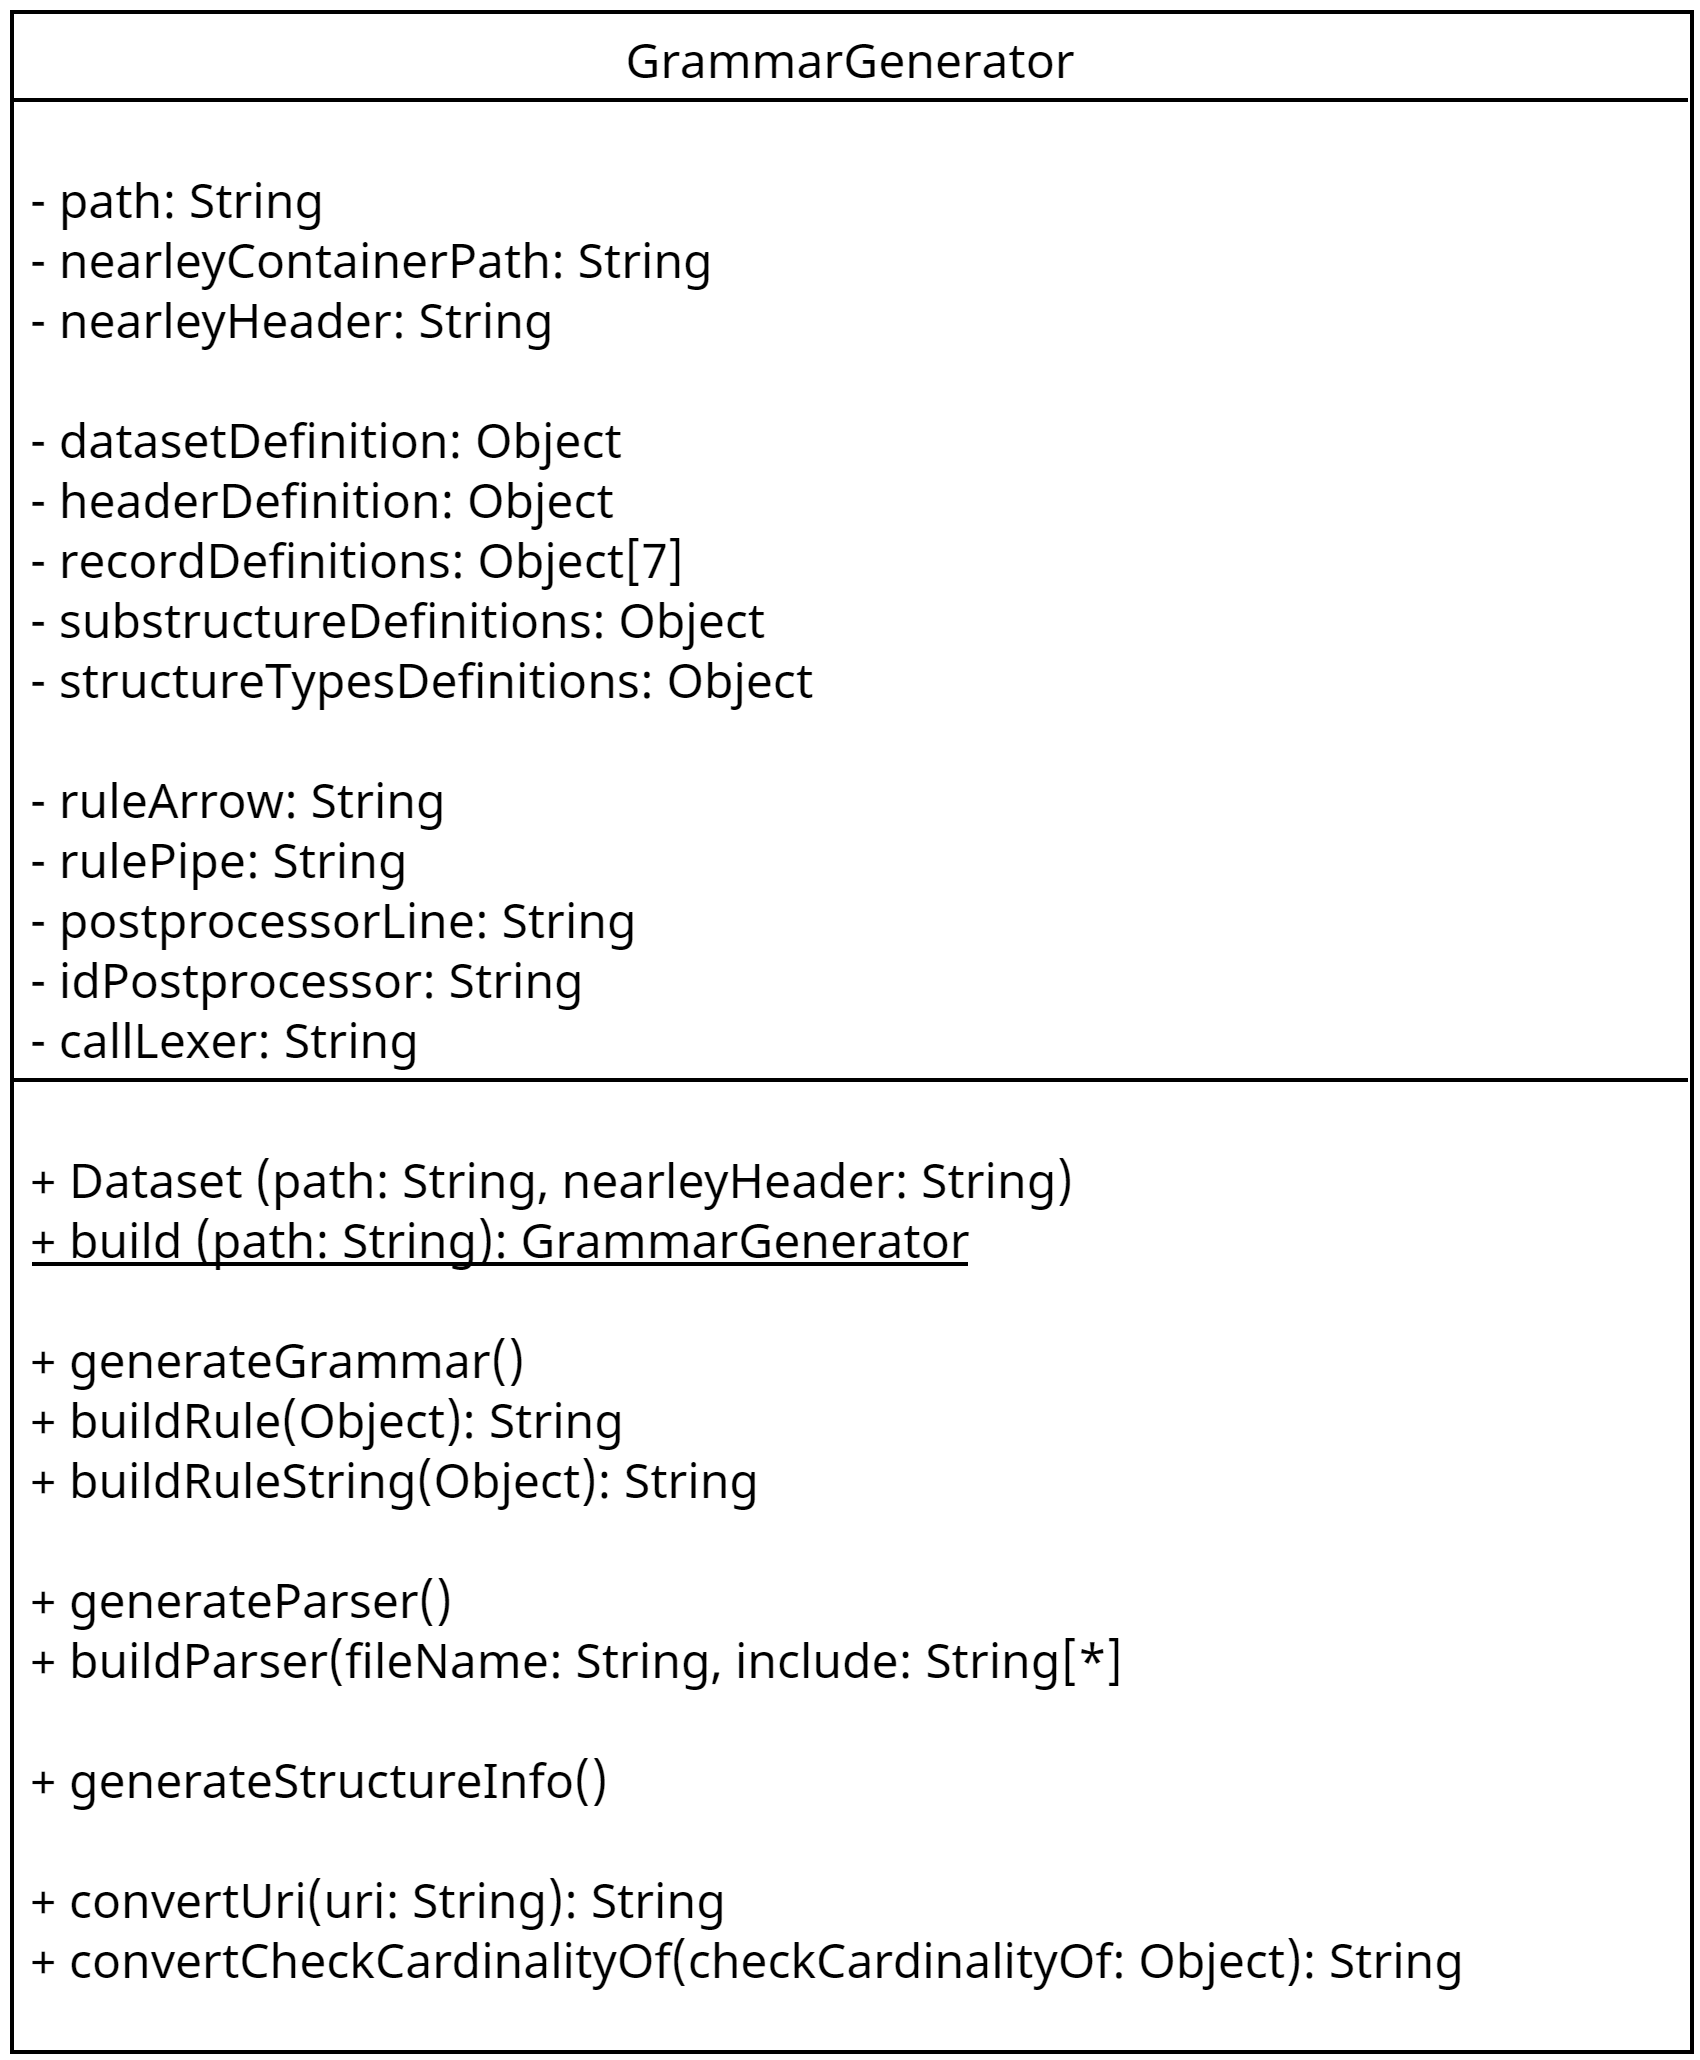
\includegraphics[width=1\textwidth]{images/UML_Class_GrammarGenerator.png}
	\caption{UML Klassendiagramm GrammarGenerator}
	\label{fig: UML Klassendiagramm GrammarGenerator}
\end{figure}

\subsection{Definition der Grammatik}
\label{subsec: Implementierung - Grammatik Generator - Definition der Grammatik}
Die Definition der Gedcom Grammatik erfolgt in Form von JavaScript Objekten. Für jede Structure, die in der Gedcom7 Spezifikation definiert ist, wird eine Grammatik Definition erstellt. Folgende Parameter sind in diesen Objekten hinterlegt:
\begin{tabular}[h]{l|l}
	URI & Die in der Gedcom7 Spezifikation für diese Structure hinterlegte URI. \\
	\hline
	lineType & Der Typ der Line einer Structure (hier wird beispielsweise hinterlegt, ob die Structure einen Cross-Reference-Identifier enthält oder auf andere Structuren verweisen darf). \\
	\hline
	Info & In der Info wird ein Informationstext zu jeder Strucutre hinterlegt. Dieser kann verwendet werden um bei Verwendung der Bibliothek dem Benutzer Informationen über die Bedeutung der Structures zukommen zu lassen.\\
	\hline
	Level & Die Levels unter denen die Structure in einer Gedcom7 Datei auftauchen kann.\\
	\hline
	Tag & Der in der Gedcom7 Spezifikation definierte Tag der Structure.\\
	\hline
	Substructs & Alle Structures, die als Substructure für eine Structure auftauchen können, inkl. der Kardinalität dieser.
\end{tabular}
\\ \\
Die Definition für einen Family Record sieht wie folgt aus. Anders als bei den Beispielen aus Abschnitt \ref{sec: Implementierung - Gedcom Grammatik} bei denen nur ein Teil der Substructures betrachtet wurde, handelt es sich hierbei um eine vollständige Definition:
\\ \\
\begin{minipage}{1.0\textwidth} \small
	\begin{lstlisting}
		{
			uri: 'g7:record-FAM',
			lineType: lineTypes.FAM_RECORD,
			info: 'Structure Info coming soon!',
			level: [0],
			tag: 'FAM',
			substructs: {
				'g7:RESN': '0:1',
				FAMILY_ATTRIBUTE_STRUCTURE: '0:M',
				FAMILY_EVENT_STRUCTURE: '0:M',
				NON_EVENT_STRUCTURE: '0:M',
				'g7:FAM-HUSB': '0:1',
				'g7:FAM-WIFE': '0:1',
				'g7:CHIL': '0:M',
				ASSOCIATION_STRUCTURE: '0:M',
				'g7:SUBM': '0:M',
				LDS_SPOUSE_SEALING: '0:M',
				IDENTIFIER_STRUCTURE: '0:M',
				NOTE_STRUCTURE: '0:M',
				SOURCE_CITATION: '0:M',
				MULTIMEDIA_LINK: '0:M',
				CHANGE_DATE: '0:1',
				CREATION_DATE: '0:1'
			}
		}
	\end{lstlisting}
	\captionof{lstlisting}{Grammatik Definition eines Family Records}
	\label{lst: Grammatik Definition Family}
\end{minipage}
\\ \\

\subsection{Grammatikgenerierung mit generateGrammar()}
\label{subsec: Implementierung - Grammatik Generator - generateGrammar}

\subsection{Parsergenerierung mit generateParser()}
\label{subsec: Implementierung - Grammatik Generator - generateParser}

\subsection{Structure Infromationen}
\label{subsec: Implementierung - Grammatik Generator - Structure Infromationen}


%========================================================================================
% SECTION: GEDCOM STRUKTUR
%========================================================================================
\section{Gedcom Struktur}
\label{sec: Implementierung - Gedcom Struktur}
% Klassendiagramm 
\subsection{Klasse \textit{Structure}}
\label{subsec: Implementierung - Gedcom Struktur - Klasse Structure}
\begin{figure}[h]
	\centering
	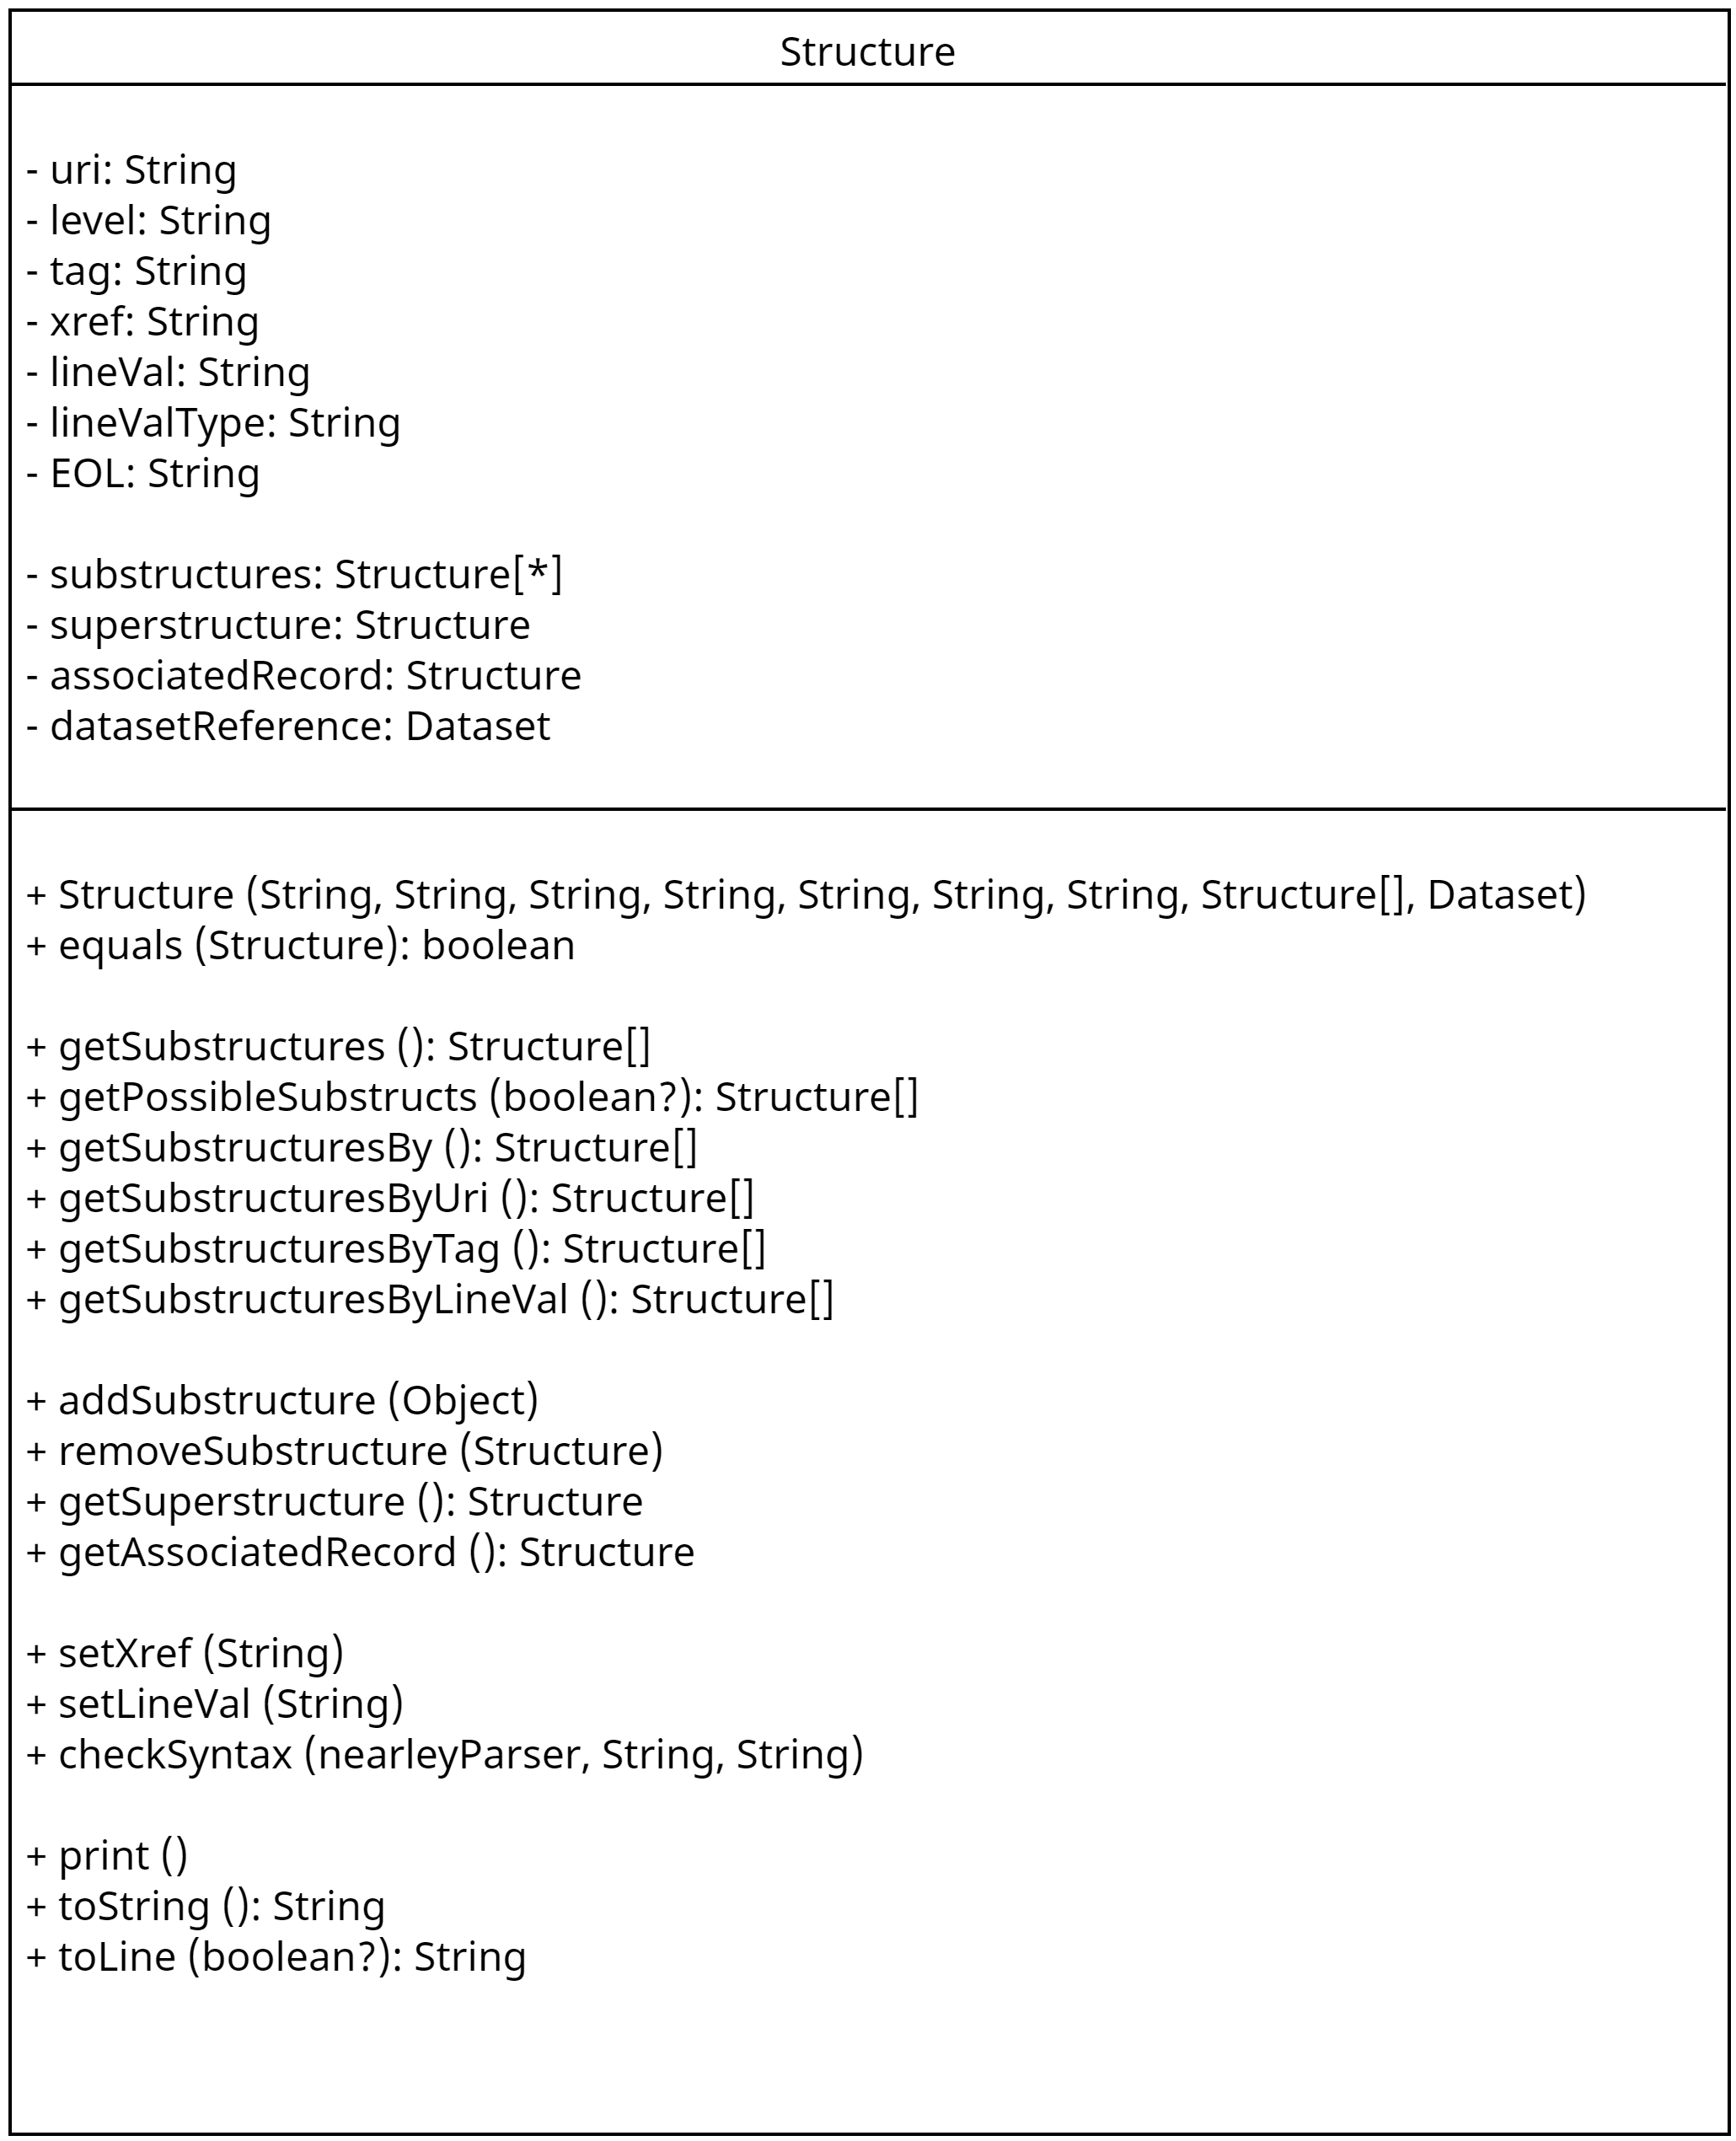
\includegraphics[width=1\textwidth]{images/UML_Class_Structure.png}
	\caption{UML Klassendiagramm Structure}
	\label{fig: UML Klassendiagramm Structure}
\end{figure}

\subsection{Klasse \textit{Record}}
\label{subsec: Implementierung - Gedcom Struktur - Klasse Record}
\begin{figure}[h]
	\centering
	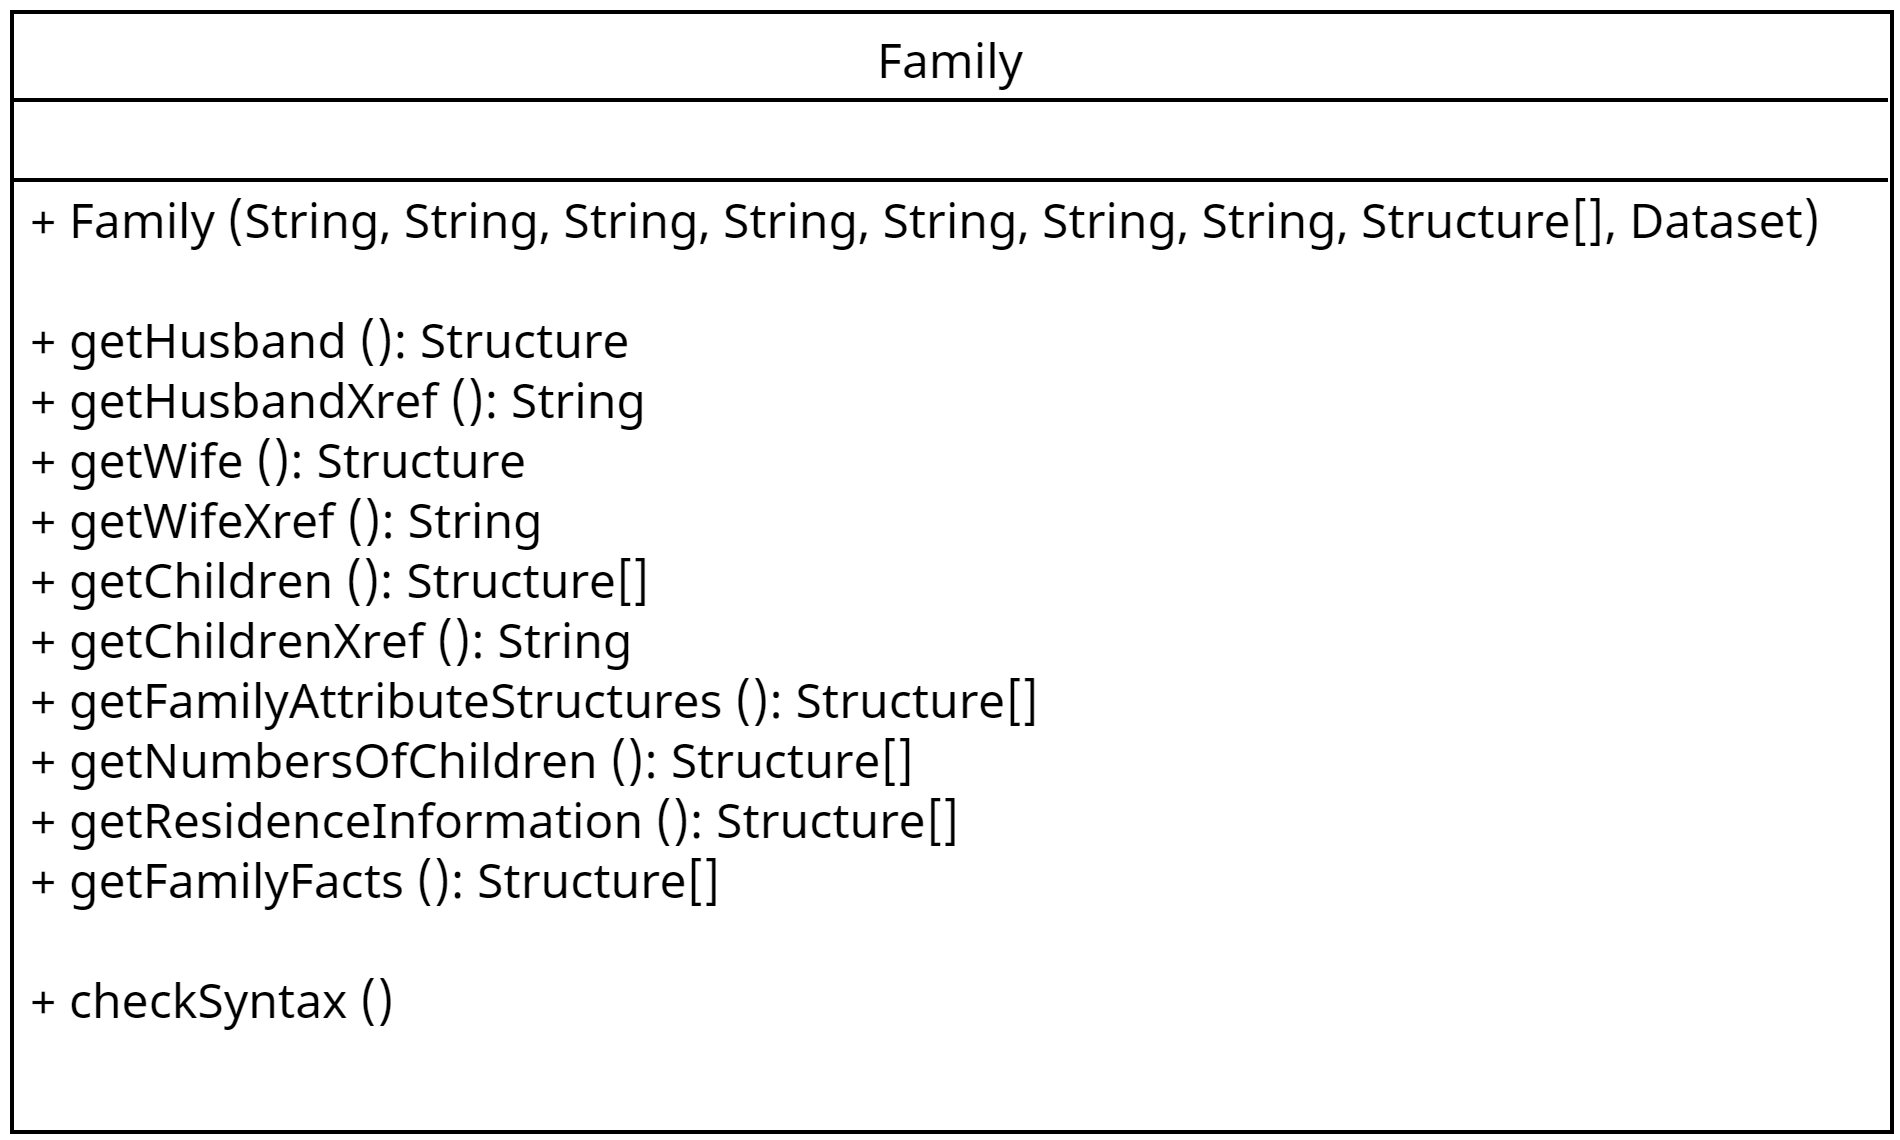
\includegraphics[width=1\textwidth]{images/UML_Class_Record.png}
	\caption{UML Klassendiagramm Record}
	\label{fig: UML Klassendiagramm Record}
\end{figure}

\subsection{Klasse \textit{Family}}
\label{subsec: Implementierung - Gedcom Struktur - Klasse Family}
\begin{figure}[h]
	\centering
	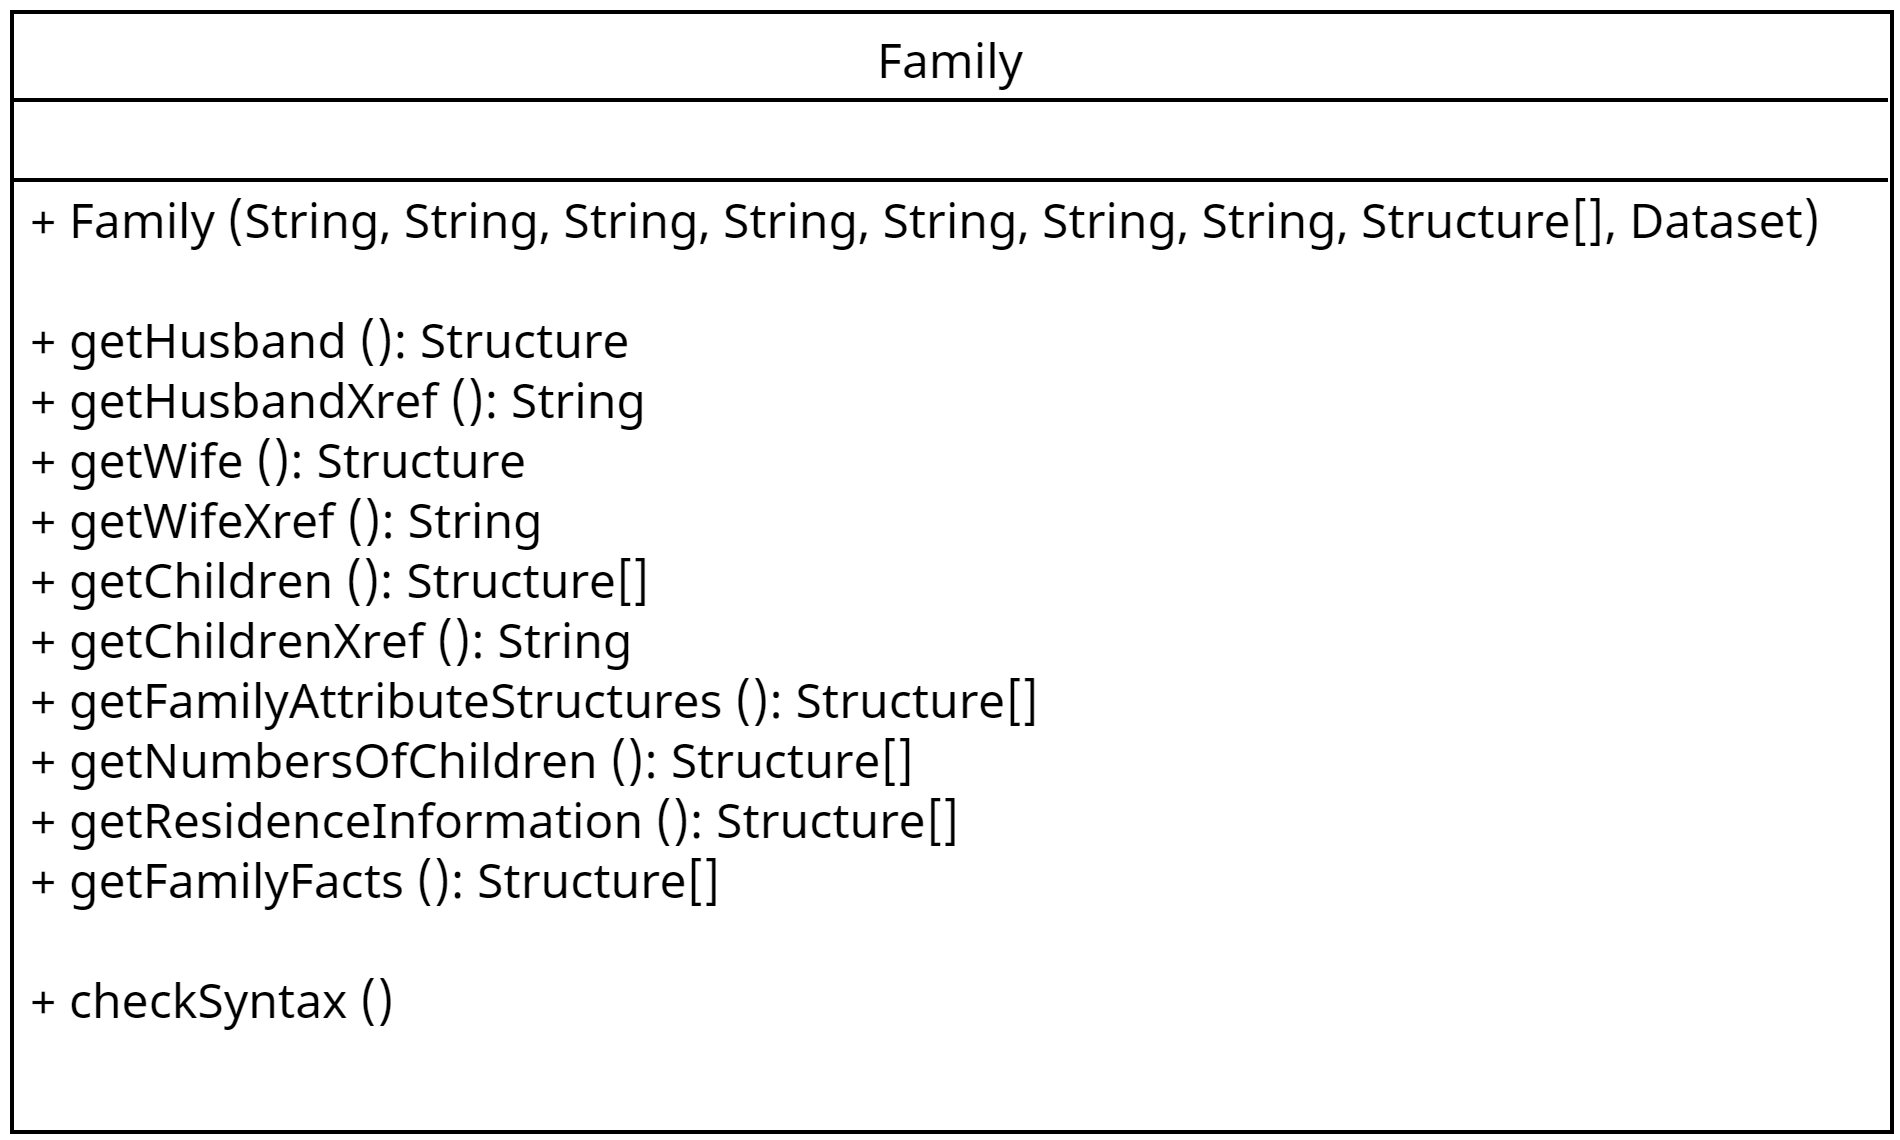
\includegraphics[width=1\textwidth]{images/UML_Class_Family.png}
	\caption{UML Klassendiagramm Family}
	\label{fig: UML Klassendiagramm Family}
\end{figure}

\subsection{Klasse \textit{Dataset}}
\label{subsec: Implementierung - Gedcom Struktur - Klasse Dataset}
\begin{figure}[h]
	\centering
	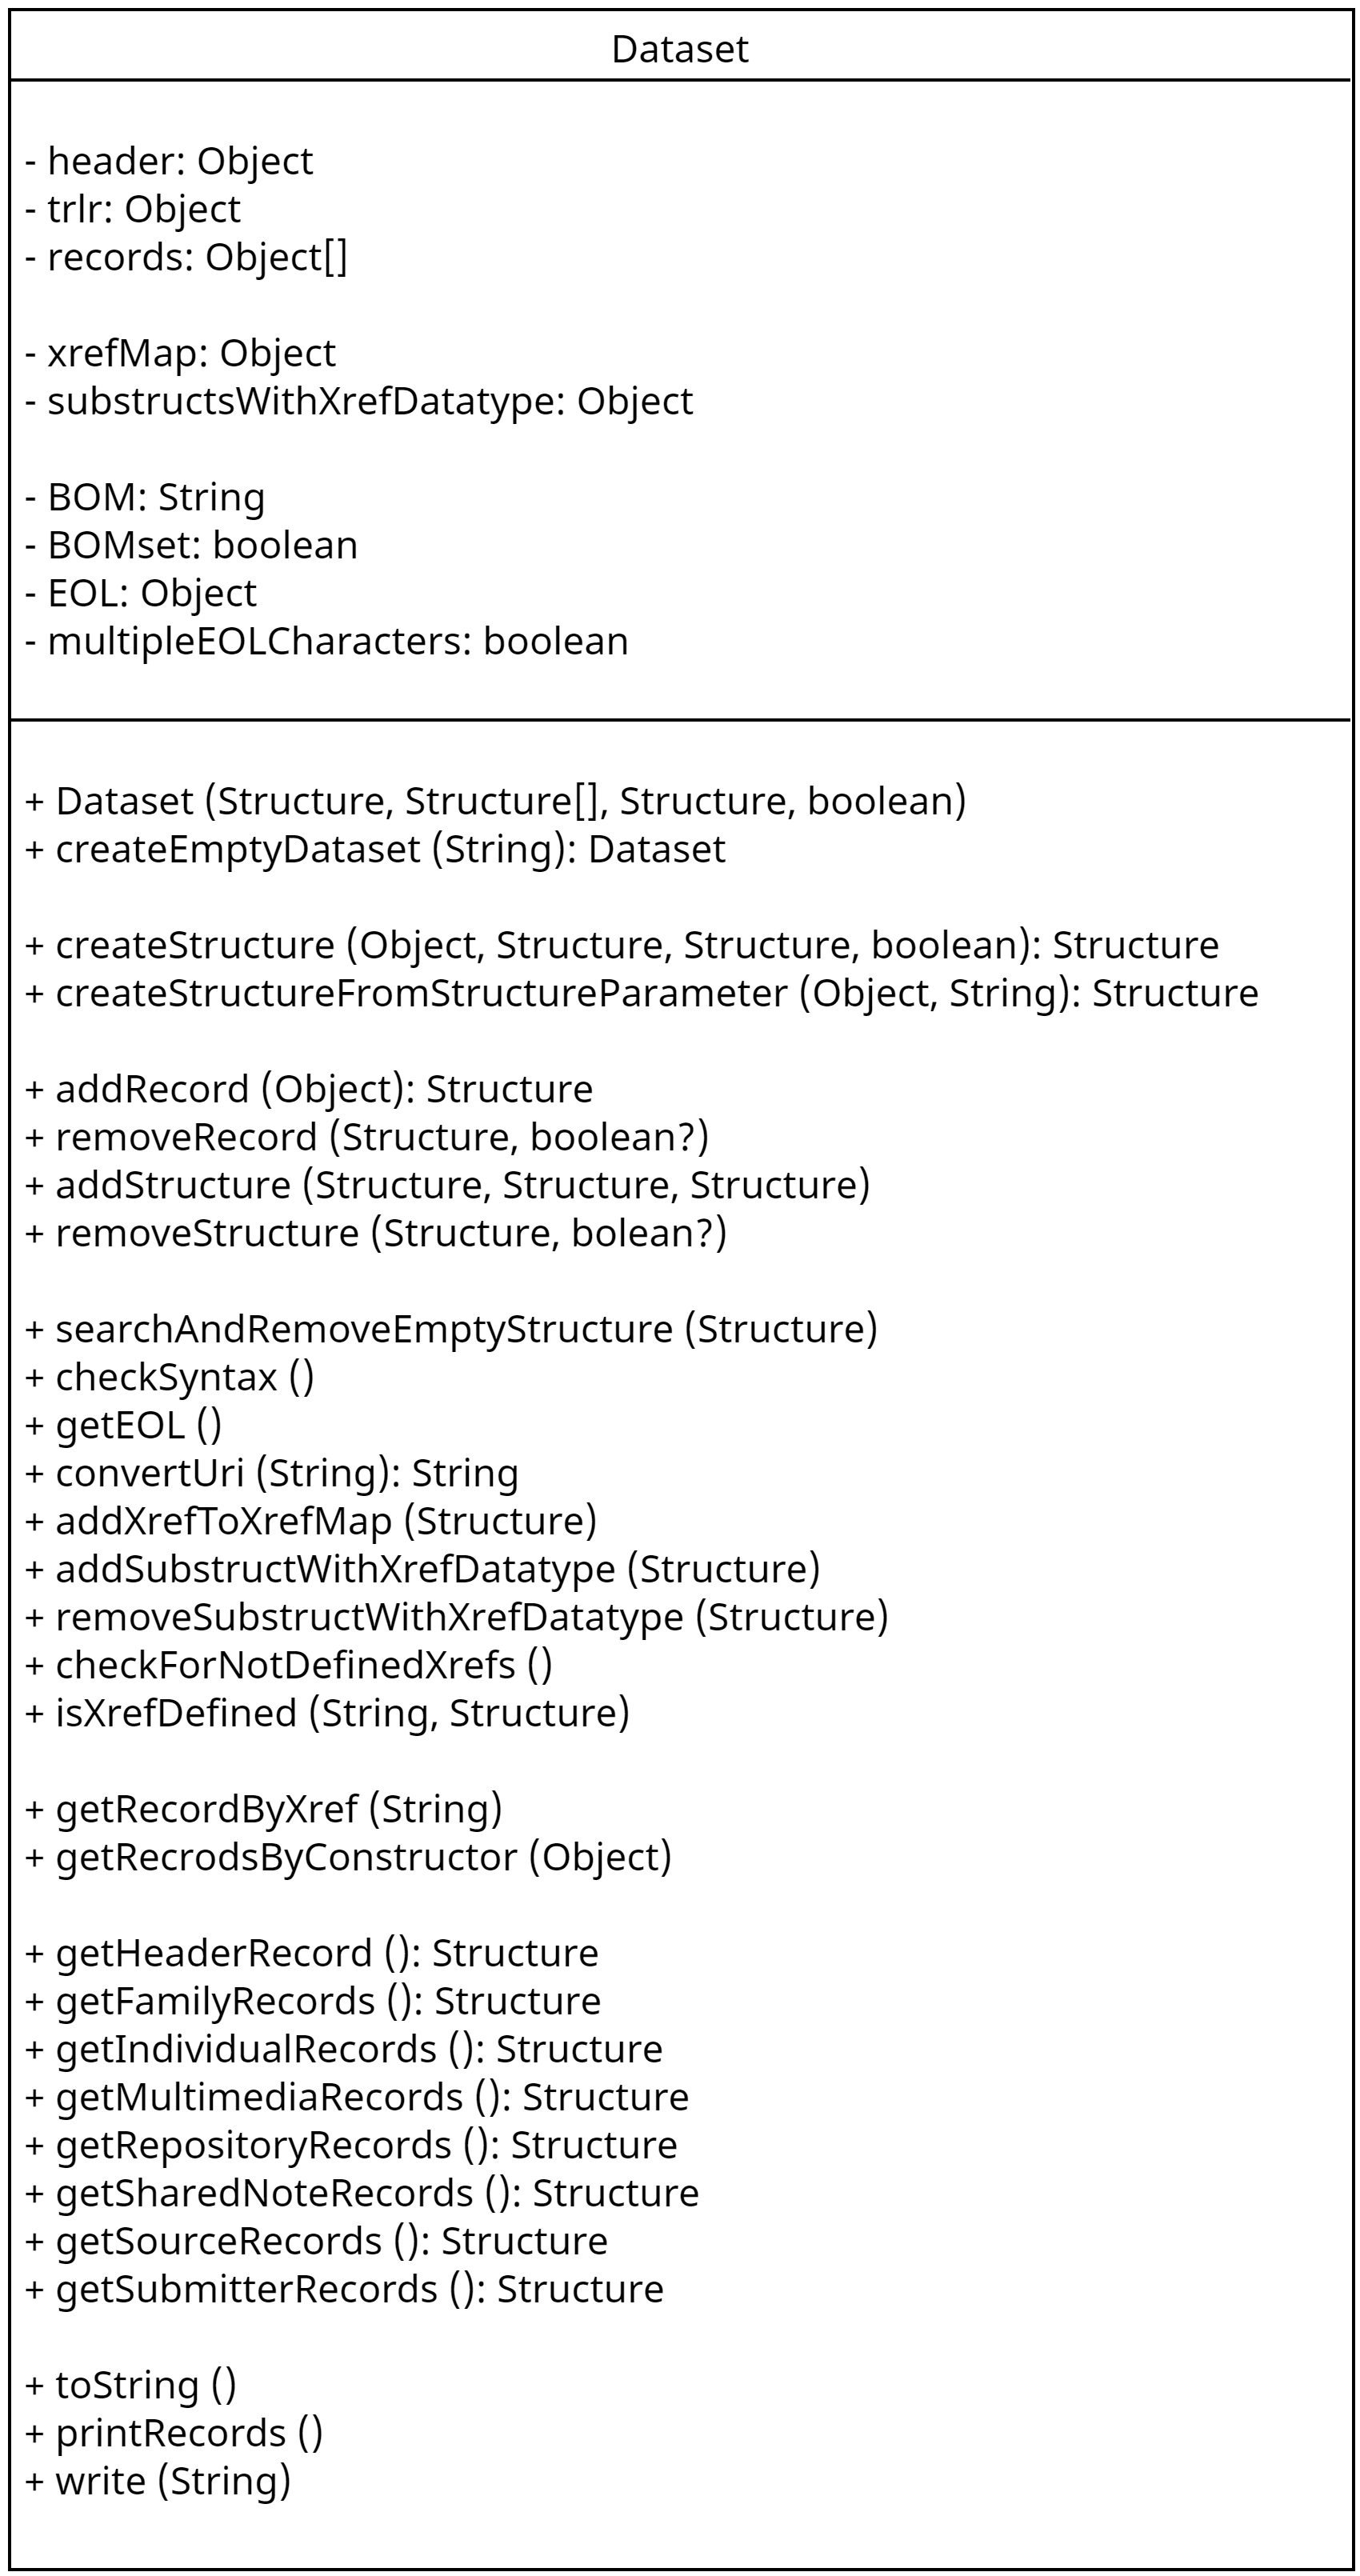
\includegraphics[width=1\textwidth]{images/UML_Class_Dataset.png}
	\caption{UML Klassendiagramm Dataset}
	\label{fig: UML Klassendiagramm Dataset}
\end{figure}


%========================================================================================
% SECTION: GEDCOM Parser
%========================================================================================
\section{Gedcom Parser}
\label{sec: Implementierung - Gedcom Parser}
% Kurze Beschreibung wie alles zusammengefügt wird
% Beispielhafter Ablauf


